\section*{Задание 1.1: Прямоугольная функция}

\textbf{Функция:}
\[
f(t) = 
\begin{cases}
a, & |t| \le b \\
0, & |t| > b
\end{cases}
\]

\textbf{Аналитическое выражение Фурье-образа:}
\[
\hat{f}(\omega) = \frac{1}{\sqrt{2\pi}} \int_{-b}^{b} a e^{-i \omega t} dt = \frac{2a}{\sqrt{2\pi}} \cdot \frac{\sin(\omega b)}{\omega}
\]

\textbf{Вывод аналитического выражения:}
\[
\hat{f}(\omega) = \frac{1}{\sqrt{2\pi}} \int_{-b}^{b} a e^{-i \omega t} dt = \frac{a}{\sqrt{2\pi}} \int_{-b}^{b} e^{-i \omega t} dt
\]
\[
= \frac{a}{\sqrt{2\pi}} \left[ \frac{e^{-i \omega t}}{-i \omega} \right]_{-b}^{b} = \frac{a}{\sqrt{2\pi}} \cdot \frac{e^{-i \omega b} - e^{i \omega b}}{-i \omega}
\]
\[
= \frac{a}{\sqrt{2\pi}} \cdot \frac{2i \sin(\omega b)}{i \omega} = \frac{2a}{\sqrt{2\pi}} \cdot \frac{\sin(\omega b)}{\omega}
\]

\textbf{Графики:}

\begin{figure}[H]
    \centering
    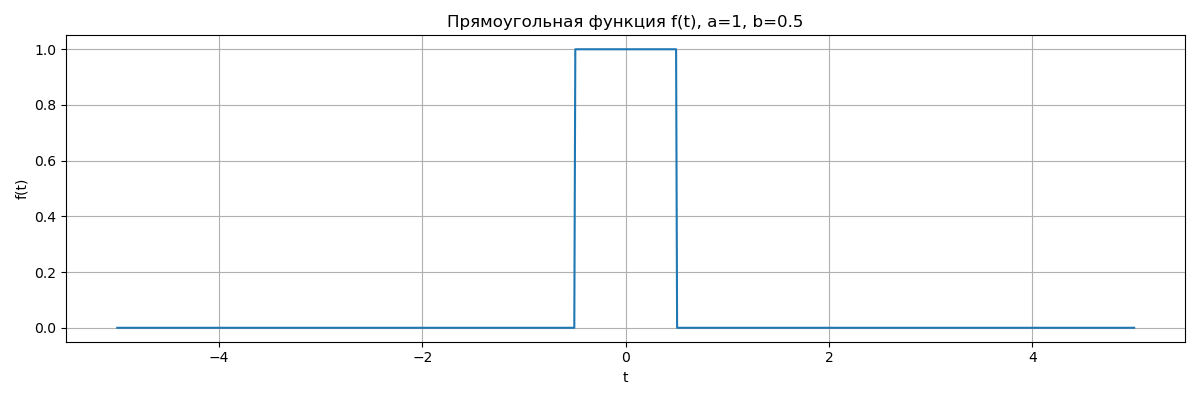
\includegraphics[width=0.8\textwidth]{rect_function_b0.5.png}
    \caption{Прямоугольная функция $f(t)$ при $b = 0.5$}
\end{figure}

\begin{figure}[H]
    \centering
    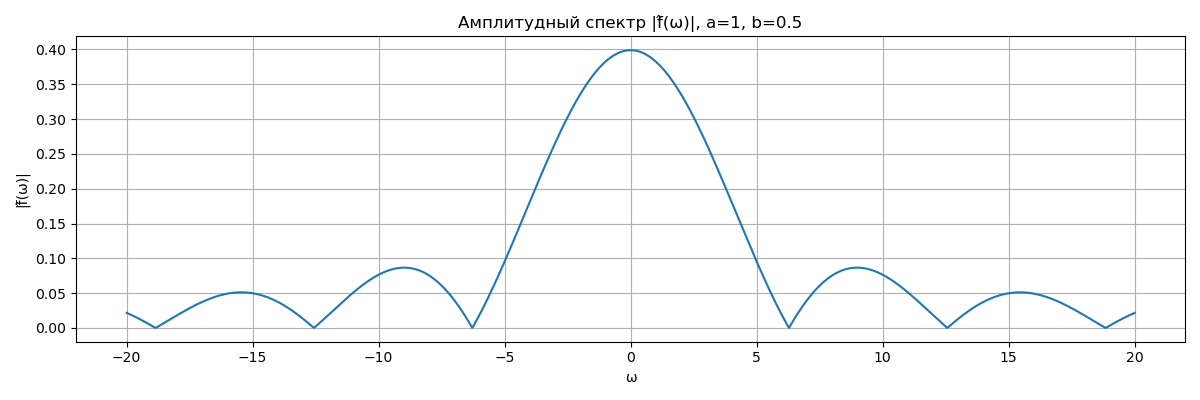
\includegraphics[width=0.8\textwidth]{rect_fourier_b0.5.png}
    \caption{Амплитудный спектр $|\hat{f}(\omega)|$ при $b = 0.5$}
\end{figure}

\begin{figure}[H]
    \centering
    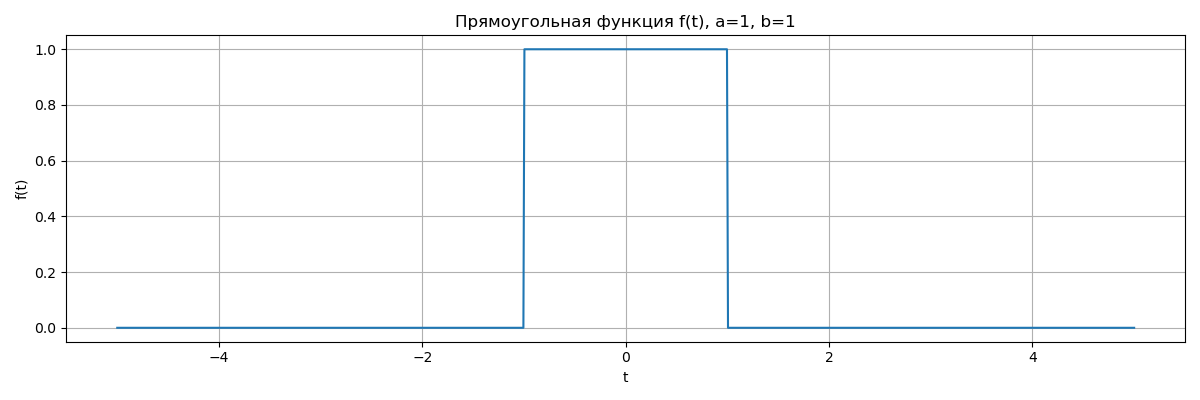
\includegraphics[width=0.8\textwidth]{rect_function_b1.png}
    \caption{Прямоугольная функция $f(t)$ при $b = 1$}
\end{figure}

\begin{figure}[H]
    \centering
    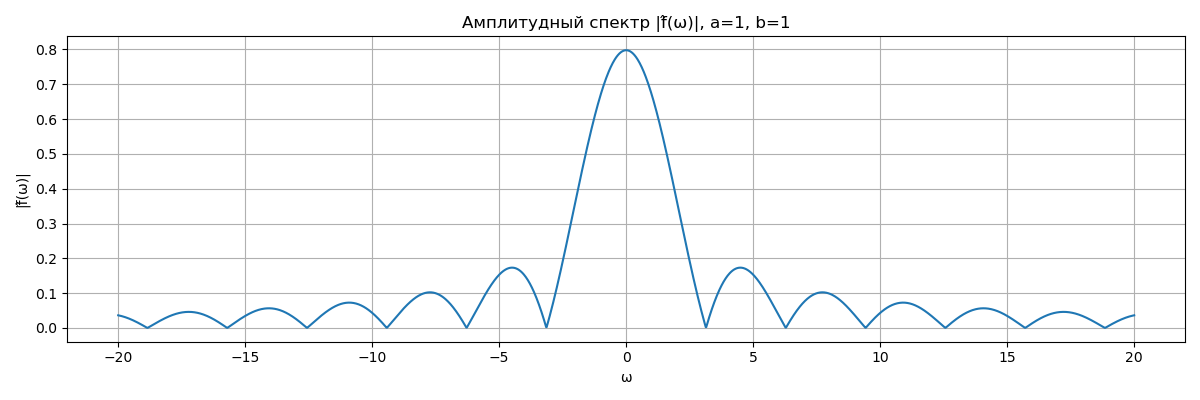
\includegraphics[width=0.8\textwidth]{rect_fourier_b1.png}
    \caption{Амплитудный спектр $|\hat{f}(\omega)|$ при $b = 1$}
\end{figure}

\begin{figure}[H]
    \centering
    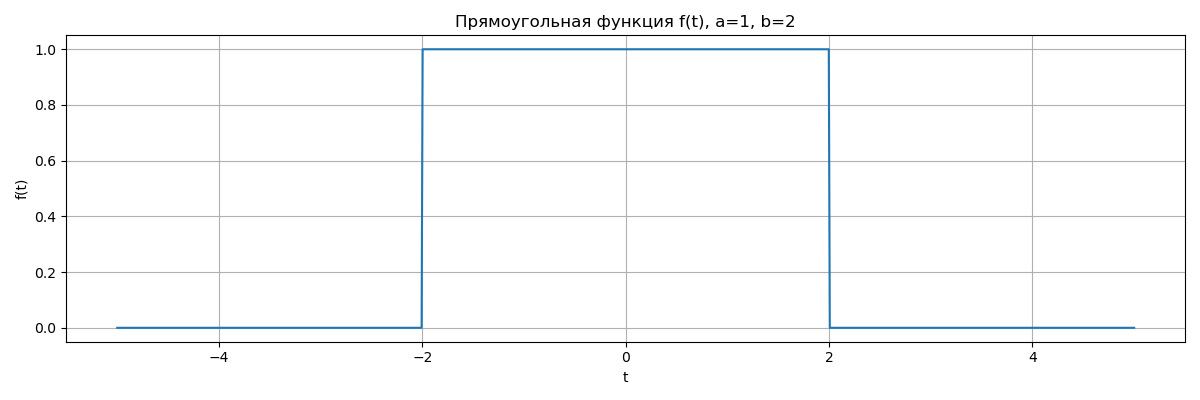
\includegraphics[width=0.8\textwidth]{rect_function_b2.png}
    \caption{Прямоугольная функция $f(t)$ при $b = 2$}
\end{figure}

\begin{figure}[H]
    \centering
    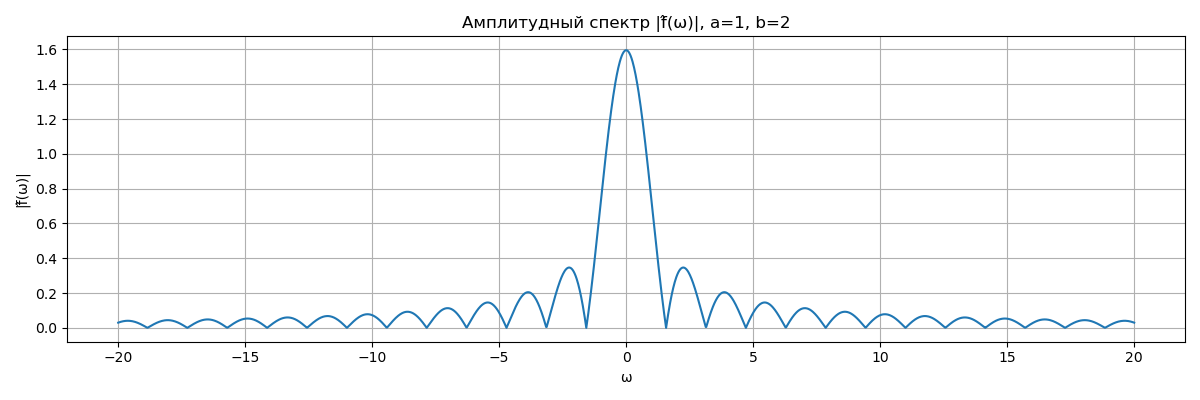
\includegraphics[width=0.8\textwidth]{rect_fourier_b2.png}
    \caption{Амплитудный спектр $|\hat{f}(\omega)|$ при $b = 2$}
\end{figure}

\textbf{Проверка равенства Парсеваля:}

Для выбранных параметров:
\begin{itemize}
    \item $\displaystyle \int_{-\infty}^{\infty} |f(t)|^2 dt \approx 2ab$
    \item $\displaystyle \int_{-\infty}^{\infty} |\hat{f}(\omega)|^2 d\omega \approx$ [значение из кода]
\end{itemize}

\textbf{Анализ:}

\begin{itemize}
    \item Увеличение $b$ растягивает $f(t)$ и сужает спектр $\hat{f}(\omega)$.
    \item Принцип неопределённости: чем шире функция во времени, тем уже спектр.
    \item Прямоугольная функция не совпадает со своим Фурье-образом, но её образ — синус-кард.
\end{itemize}


\section*{Задание 1.2: Треугольная функция}

\textbf{Функция:}
\[
f(t) = 
\begin{cases}
a - \frac{a |t|}{b}, & |t| \le b \\
0, & |t| > b
\end{cases}
\]

\textbf{Аналитическое выражение Фурье-образа:}
\[
\hat{f}(\omega) = \frac{2a}{\sqrt{2\pi}} \cdot \frac{1 - \cos(\omega b)}{\omega^2 b}
\]

\textbf{Вывод аналитического выражения:}
\[
\hat{f}(\omega) = \frac{1}{\sqrt{2\pi}} \int_{-b}^{b} \left(a - \frac{a |t|}{b}\right) e^{-i \omega t} dt
\]
\[
= \frac{a}{\sqrt{2\pi}} \int_{-b}^{b} e^{-i \omega t} dt - \frac{a}{b\sqrt{2\pi}} \int_{-b}^{b} |t| e^{-i \omega t} dt
\]
\[
= \frac{2a}{\sqrt{2\pi}} \cdot \frac{\sin(\omega b)}{\omega} - \frac{2a}{b\sqrt{2\pi}} \int_{0}^{b} t \cos(\omega t) dt
\]
\[
= \frac{2a}{\sqrt{2\pi}} \cdot \frac{\sin(\omega b)}{\omega} - \frac{2a}{b\sqrt{2\pi}} \cdot \frac{b \cos(\omega b) + \omega b \sin(\omega b) - 1}{\omega^2}
\]
\[
= \frac{2a}{\sqrt{2\pi}} \cdot \frac{1 - \cos(\omega b)}{\omega^2 b}
\]

\textbf{Графики:}

\begin{figure}[H]
    \centering
    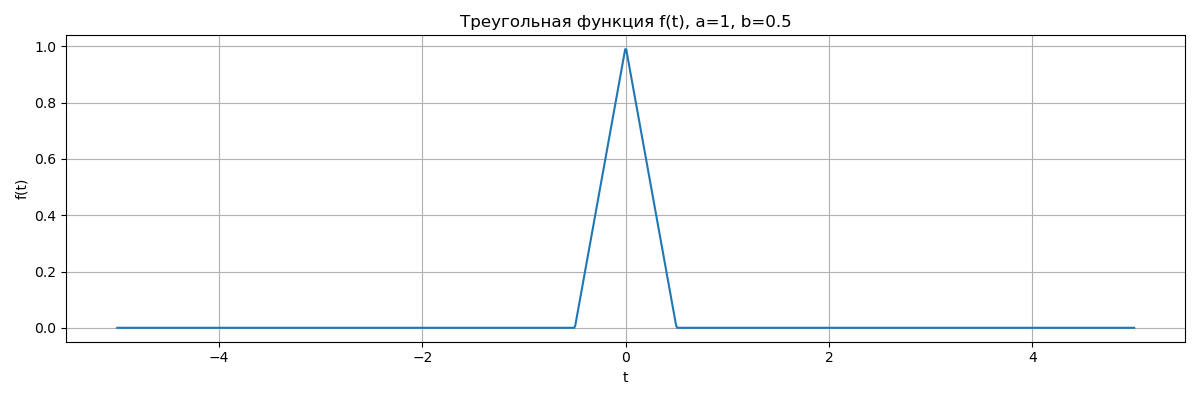
\includegraphics[width=0.8\textwidth]{triangle_function_b0.5.png}
    \caption{Треугольная функция $f(t)$ при $b = 0.5$}
\end{figure}

\begin{figure}[H]
    \centering
    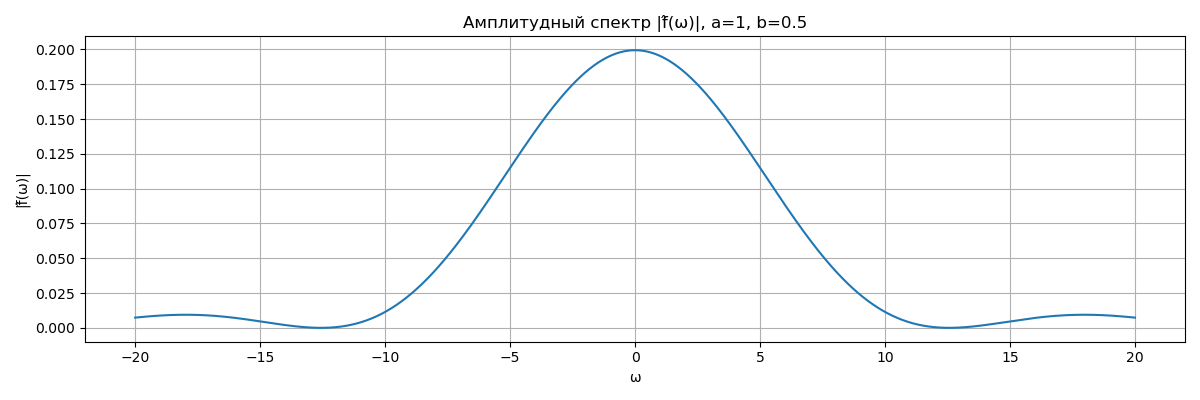
\includegraphics[width=0.8\textwidth]{triangle_spectrum_b0.5.png}
    \caption{Амплитудный спектр $|\hat{f}(\omega)|$ при $b = 0.5$}
\end{figure}

\begin{figure}[H]
    \centering
    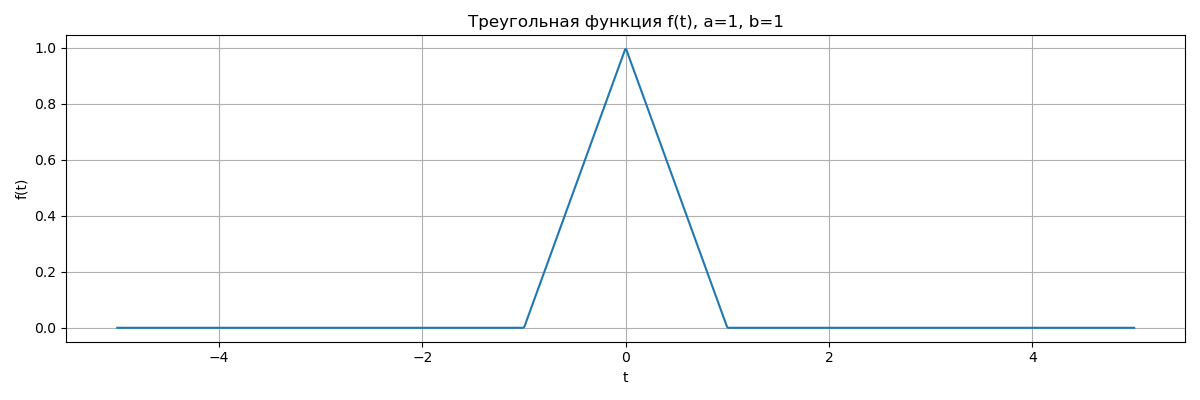
\includegraphics[width=0.8\textwidth]{triangle_function_b1.png}
    \caption{Треугольная функция $f(t)$ при $b = 1$}
\end{figure}

\begin{figure}[H]
    \centering
    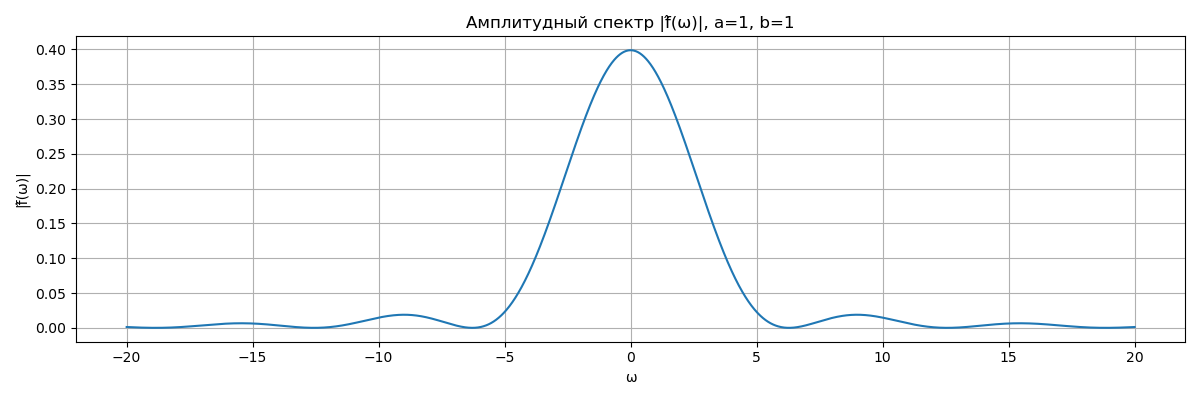
\includegraphics[width=0.8\textwidth]{triangle_spectrum_b1.png}
    \caption{Амплитудный спектр $|\hat{f}(\omega)|$ при $b = 1$}
\end{figure}

\begin{figure}[H]
    \centering
    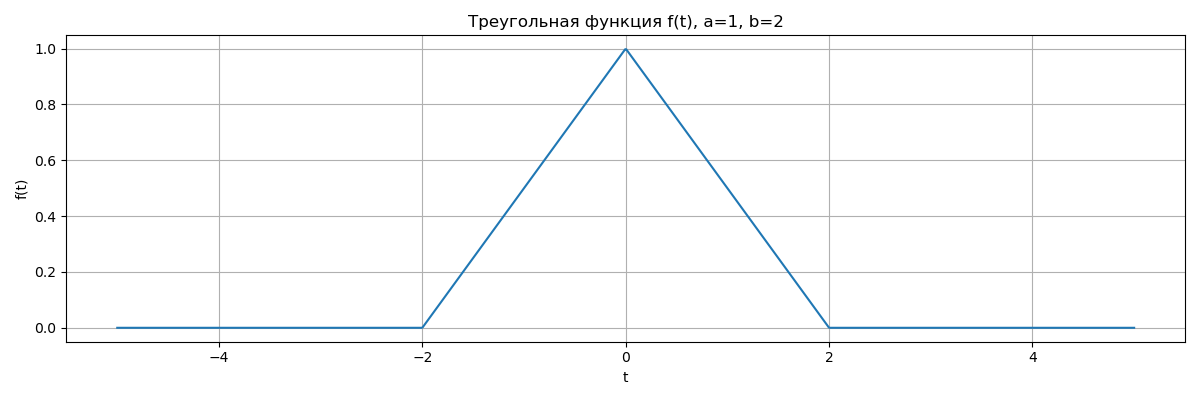
\includegraphics[width=0.8\textwidth]{triangle_function_b2.png}
    \caption{Треугольная функция $f(t)$ при $b = 2$}
\end{figure}

\begin{figure}[H]
    \centering
    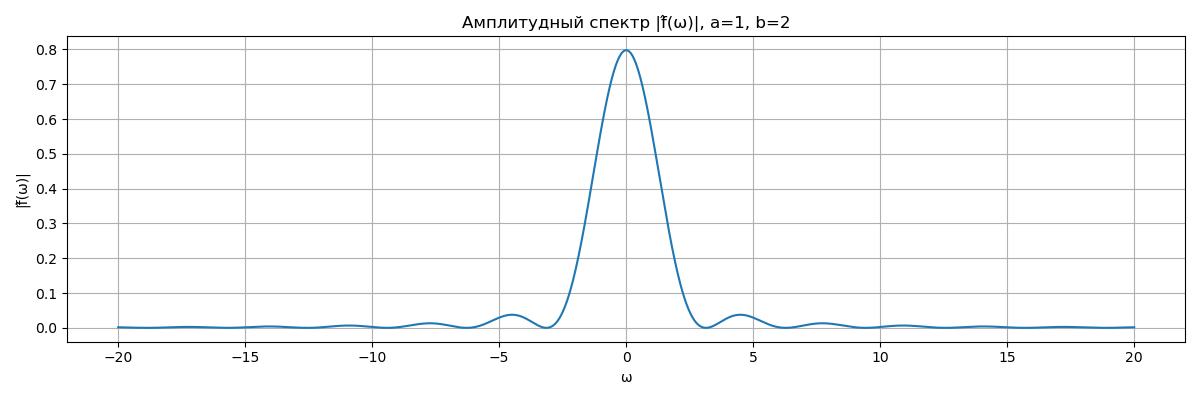
\includegraphics[width=0.8\textwidth]{triangle_spectrum_b2.png}
    \caption{Амплитудный спектр $|\hat{f}(\omega)|$ при $b = 2$}
\end{figure}

\textbf{Проверка равенства Парсеваля:}

\begin{itemize}
    \item Теоретическое значение: $\displaystyle \int |f(t)|^2 dt = \frac{2 a^2 b}{3}$
    \item Численный результат: см. выводы кода
\end{itemize}

\textbf{Анализ:}

\begin{itemize}
    \item Более гладкая функция → спектр быстрее убывает.
    \item Принцип неопределённости проявляется: при увеличении $b$ спектр сужается.
\end{itemize}

\section*{Задание 1.3: Кардинальный синус}

\textbf{Функция:}
\[
f(t) = a \cdot \mathrm{sinc}(bt) = a \cdot \frac{\sin(\pi b t)}{\pi b t}
\]

\textbf{Фурье-образ:}
\[
\hat{f}(\omega) = \frac{a}{\sqrt{2\pi}} \cdot \chi_{[-\pi b, \pi b]}(\omega)
\]

\textbf{Графики:}

\begin{figure}[H]
    \centering
    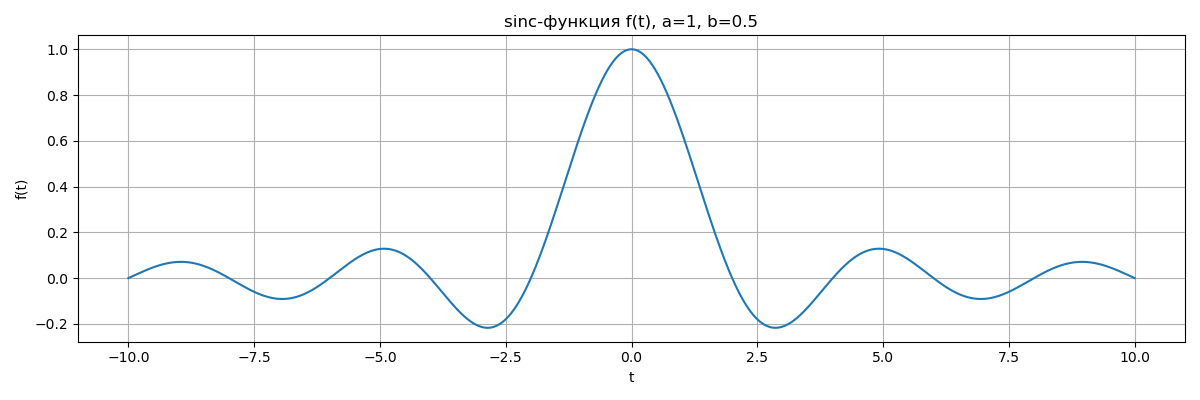
\includegraphics[width=0.8\textwidth]{sinc_function_b0.5.png}
    \caption{Функция $f(t) = a \cdot \mathrm{sinc}(bt)$ при $b = 0.5$}
\end{figure}

\begin{figure}[H]
    \centering
    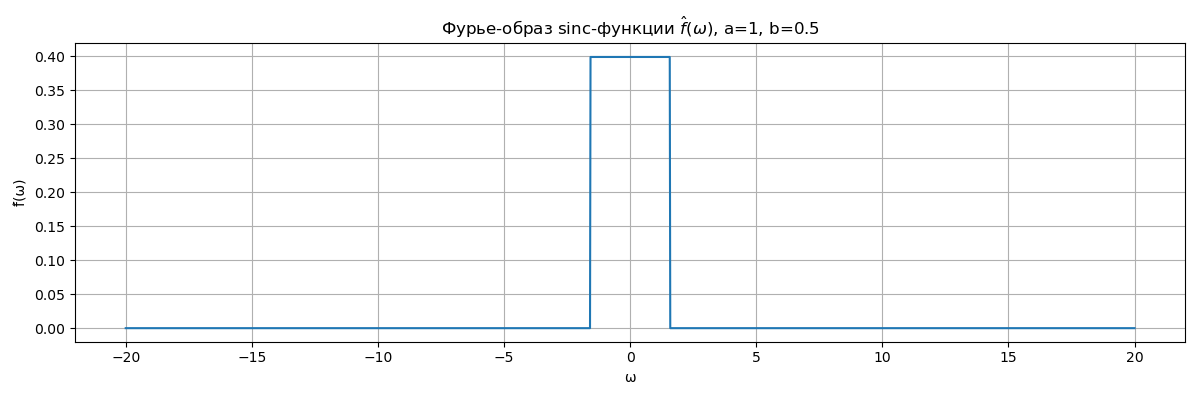
\includegraphics[width=0.8\textwidth]{sinc_spectrum_b0.5.png}
    \caption{Фурье-образ $\hat{f}(\omega)$ — прямоугольная функция при $b = 0.5$}
\end{figure}

\begin{figure}[H]
    \centering
    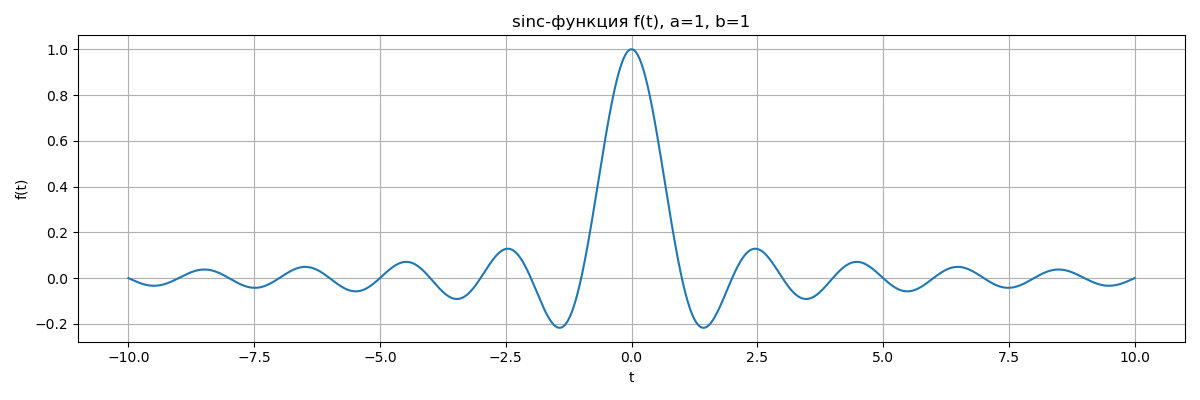
\includegraphics[width=0.8\textwidth]{sinc_function_b1.png}
    \caption{Функция $f(t) = a \cdot \mathrm{sinc}(bt)$ при $b = 1$}
\end{figure}

\begin{figure}[H]
    \centering
    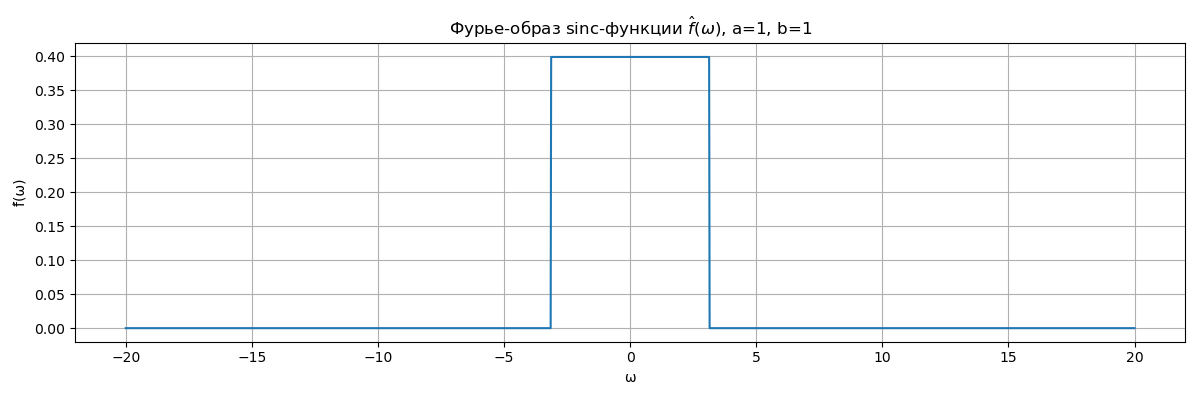
\includegraphics[width=0.8\textwidth]{sinc_spectrum_b1.png}
    \caption{Фурье-образ $\hat{f}(\omega)$ — прямоугольная функция при $b = 1$}
\end{figure}

\begin{figure}[H]
    \centering
    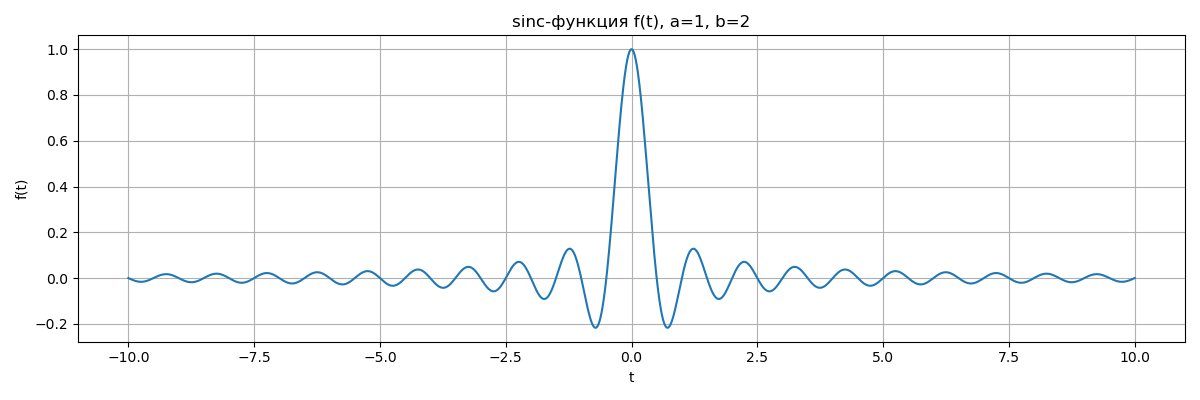
\includegraphics[width=0.8\textwidth]{sinc_function_b2.png}
    \caption{Функция $f(t) = a \cdot \mathrm{sinc}(bt)$ при $b = 2$}
\end{figure}

\begin{figure}[H]
    \centering
    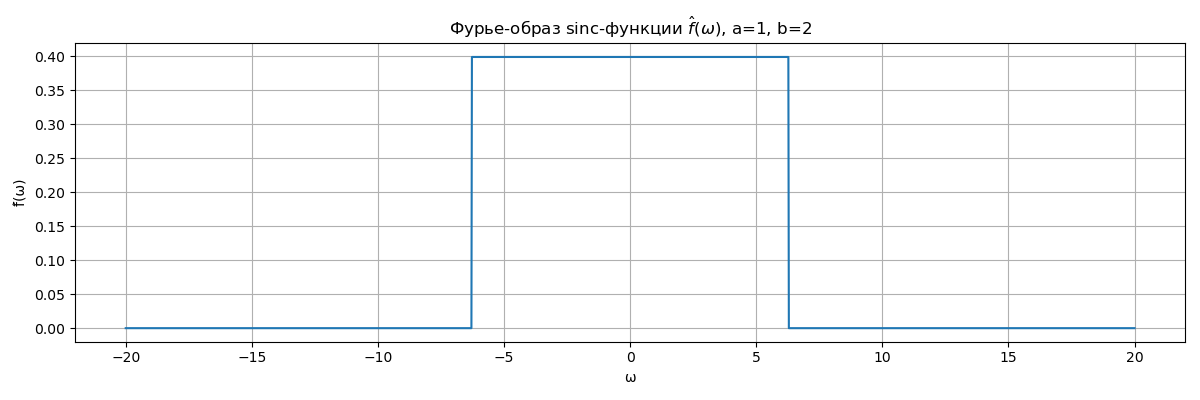
\includegraphics[width=0.8\textwidth]{sinc_spectrum_b2.png}
    \caption{Фурье-образ $\hat{f}(\omega)$ — прямоугольная функция при $b = 2$}
\end{figure}

\textbf{Проверка равенства Парсеваля:}

\begin{itemize}
    \item Теоретически: $\displaystyle \int_{-\infty}^{\infty} |f(t)|^2 dt = \frac{a^2}{b}$
    \item Численно: см. Python-вывод
\end{itemize}

\textbf{Анализ:}

\begin{itemize}
    \item sinc-функция — основа многих Фурье-преобразований.
    \item Ширина sinc обратно пропорциональна ширине спектра.
    \item Чем "длиннее" sinc, тем "уже" прямоугольный спектр.
\end{itemize}

\section*{Задание 1.4: Функция Гаусса}

\textbf{Функция:}
\[
f(t) = a \cdot e^{-b t^2}
\]

\textbf{Фурье-образ:}
\[
\hat{f}(\omega) = \frac{a}{\sqrt{2b}} \cdot e^{-\frac{\omega^2}{4b}}
\]

\textbf{Графики:}

\begin{figure}[H]
    \centering
    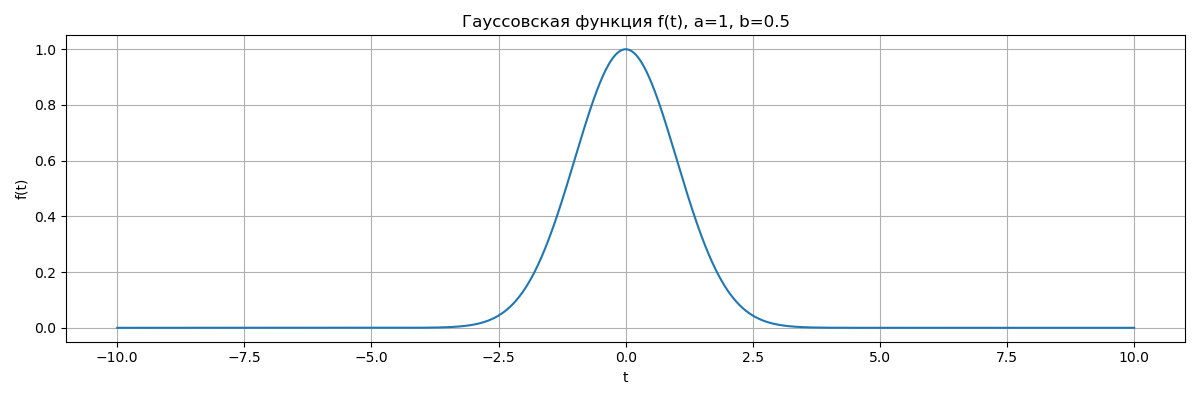
\includegraphics[width=0.8\textwidth]{gauss_function_b0.5.png}
    \caption{Гауссовская функция $f(t)$ при $b = 0.5$}
\end{figure}

\begin{figure}[H]
    \centering
    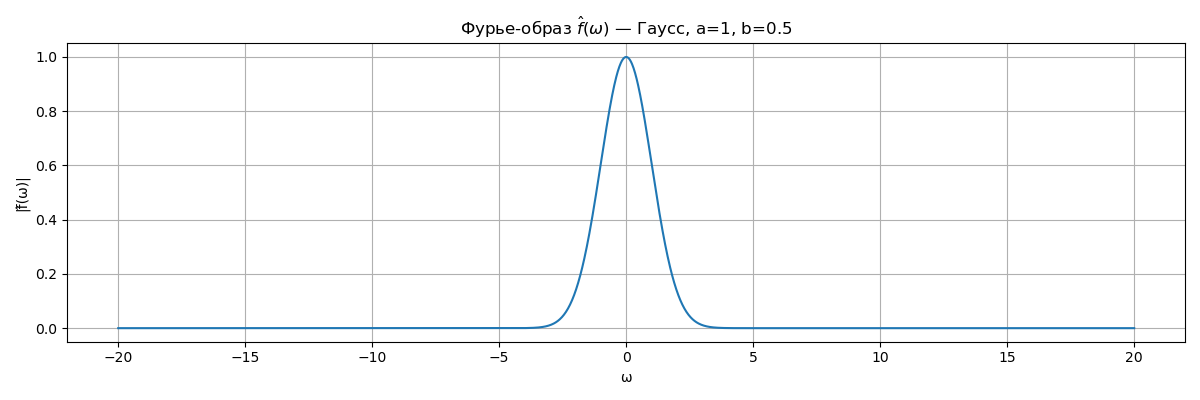
\includegraphics[width=0.8\textwidth]{gauss_spectrum_b0.5.png}
    \caption{Фурье-образ $\hat{f}(\omega)$ — тоже Гаусс при $b = 0.5$}
\end{figure}

\begin{figure}[H]
    \centering
    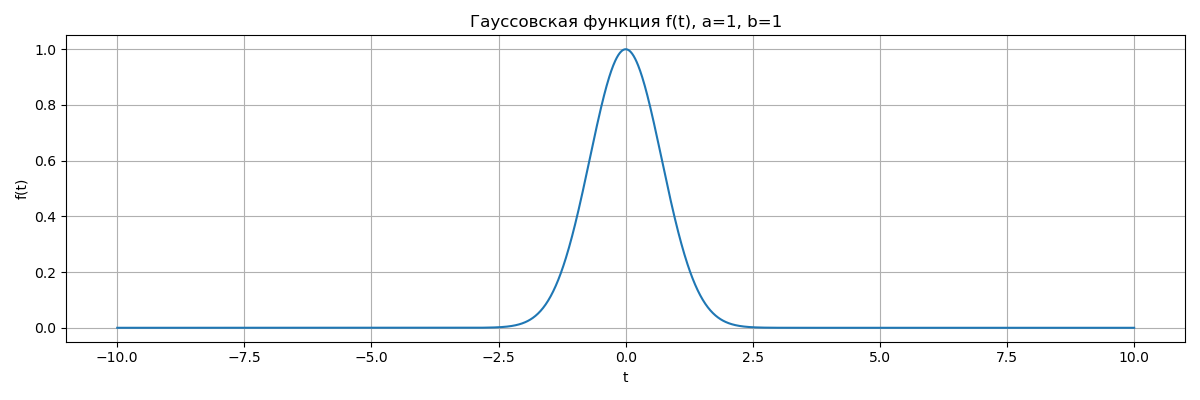
\includegraphics[width=0.8\textwidth]{gauss_function_b1.png}
    \caption{Гауссовская функция $f(t)$ при $b = 1$}
\end{figure}

\begin{figure}[H]
    \centering
    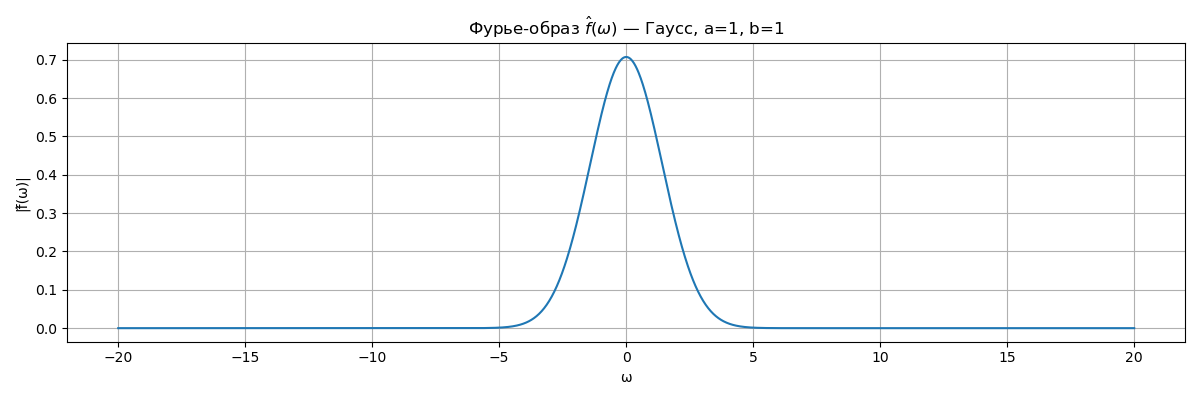
\includegraphics[width=0.8\textwidth]{gauss_spectrum_b1.png}
    \caption{Фурье-образ $\hat{f}(\omega)$ — тоже Гаусс при $b = 1$}
\end{figure}

\begin{figure}[H]
    \centering
    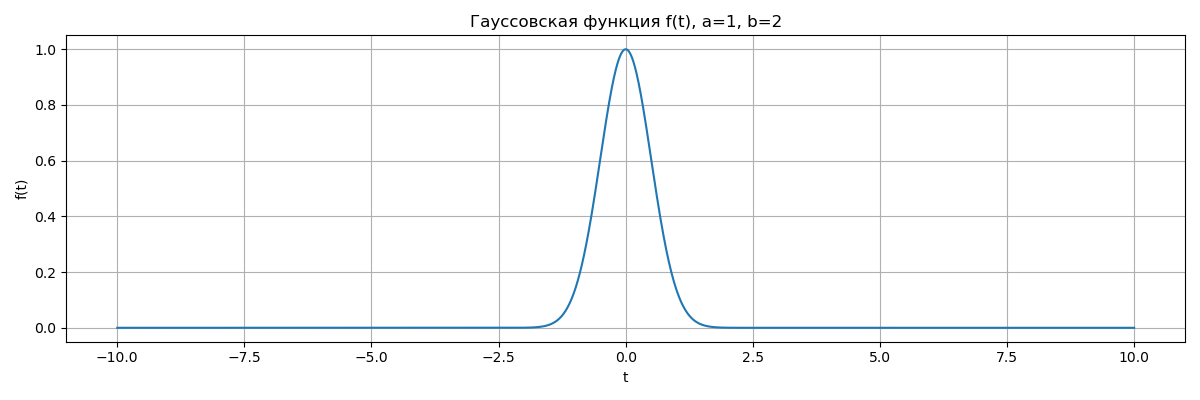
\includegraphics[width=0.8\textwidth]{gauss_function_b2.png}
    \caption{Гауссовская функция $f(t)$ при $b = 2$}
\end{figure}

\begin{figure}[H]
    \centering
    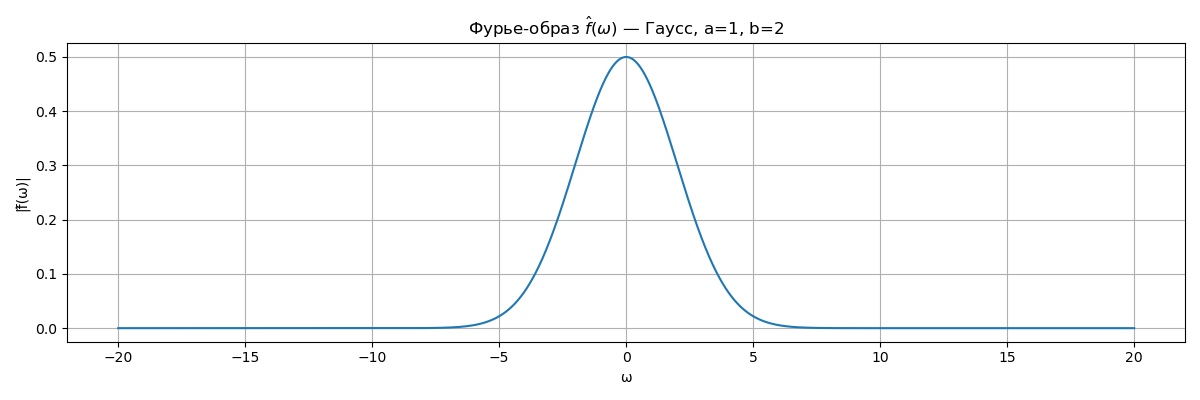
\includegraphics[width=0.8\textwidth]{gauss_spectrum_b2.png}
    \caption{Фурье-образ $\hat{f}(\omega)$ — тоже Гаусс при $b = 2$}
\end{figure}

\textbf{Проверка равенства Парсеваля:}

\begin{itemize}
    \item Теоретически: $\displaystyle \int |f(t)|^2 dt = a^2 \cdot \sqrt{\frac{\pi}{2b}}$
    \item Практически: см. численные результаты
\end{itemize}

\textbf{Анализ:}

\begin{itemize}
    \item Гаусс — единственная функция, совпадающая со своим Фурье-образу (до масштаба).
    \item Чем уже $f(t)$, тем шире спектр — яркий пример принципа неопределённости.
\end{itemize}

\section*{Задание 1.5: Двустороннее затухание}

\textbf{Функция:}
\[
f(t) = a \cdot e^{-b |t|}
\]

\textbf{Фурье-образ:}
\[
\hat{f}(\omega) = \frac{2ab}{\sqrt{2\pi}(b^2 + \omega^2)}
\]

\textbf{Вывод аналитического выражения:}
\[
\hat{f}(\omega) = \frac{1}{\sqrt{2\pi}} \int_{-\infty}^{\infty} a e^{-b |t|} e^{-i \omega t} dt
\]
\[
= \frac{a}{\sqrt{2\pi}} \left( \int_{-\infty}^{0} e^{b t} e^{-i \omega t} dt + \int_{0}^{\infty} e^{-b t} e^{-i \omega t} dt \right)
\]
\[
= \frac{a}{\sqrt{2\pi}} \left( \int_{-\infty}^{0} e^{(b - i \omega) t} dt + \int_{0}^{\infty} e^{-(b + i \omega) t} dt \right)
\]
\[
= \frac{a}{\sqrt{2\pi}} \left( \frac{1}{b - i \omega} + \frac{1}{b + i \omega} \right)
\]
\[
= \frac{a}{\sqrt{2\pi}} \cdot \frac{2b}{b^2 + \omega^2} = \frac{2ab}{\sqrt{2\pi}(b^2 + \omega^2)}
\]

\textbf{Графики:}

\begin{figure}[H]
    \centering
    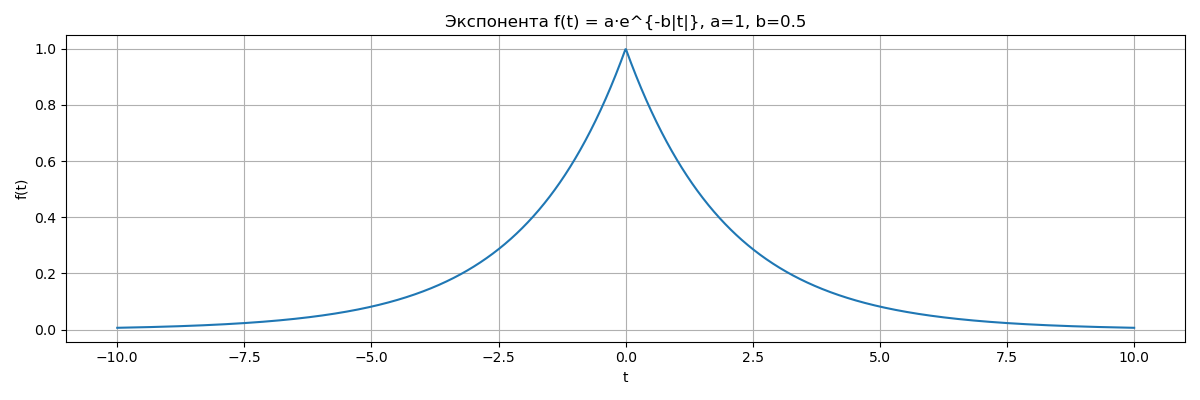
\includegraphics[width=0.8\textwidth]{exp_function_b0.5.png}
    \caption{Экспоненциальная функция $f(t)$ при $b = 0.5$}
\end{figure}

\begin{figure}[H]
    \centering
    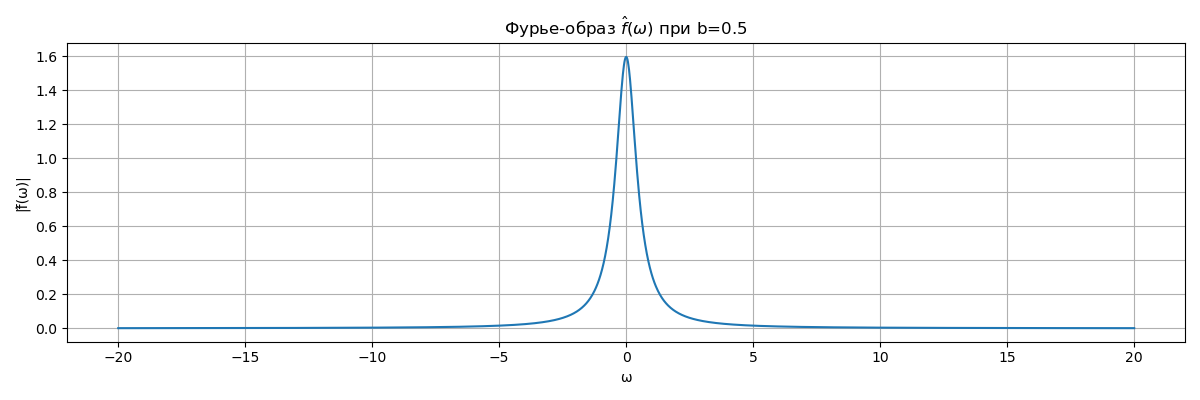
\includegraphics[width=0.8\textwidth]{exp_spectrum_b0.5.png}
    \caption{Спектр $\hat{f}(\omega)$ — функция Лоренца при $b = 0.5$}
\end{figure}

\begin{figure}[H]
    \centering
    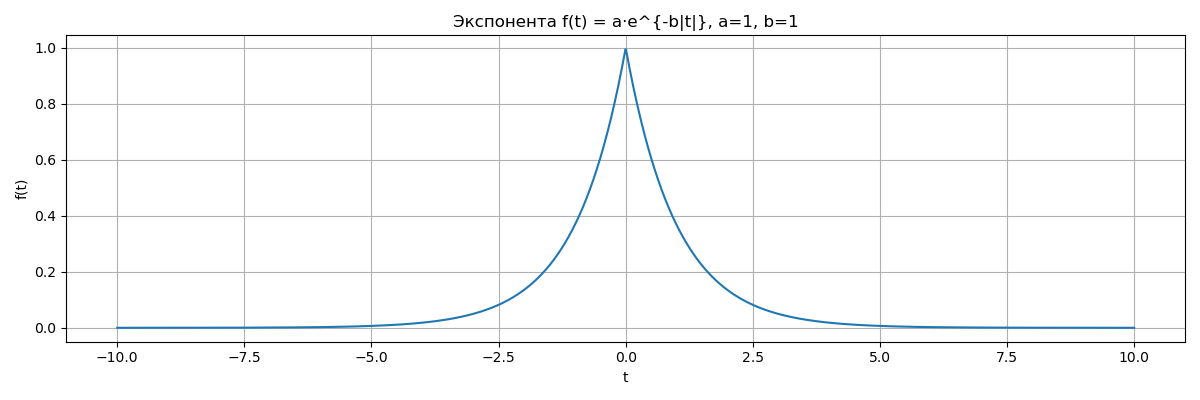
\includegraphics[width=0.8\textwidth]{exp_function_b1.png}
    \caption{Экспоненциальная функция $f(t)$ при $b = 1$}
\end{figure}

\begin{figure}[H]
    \centering
    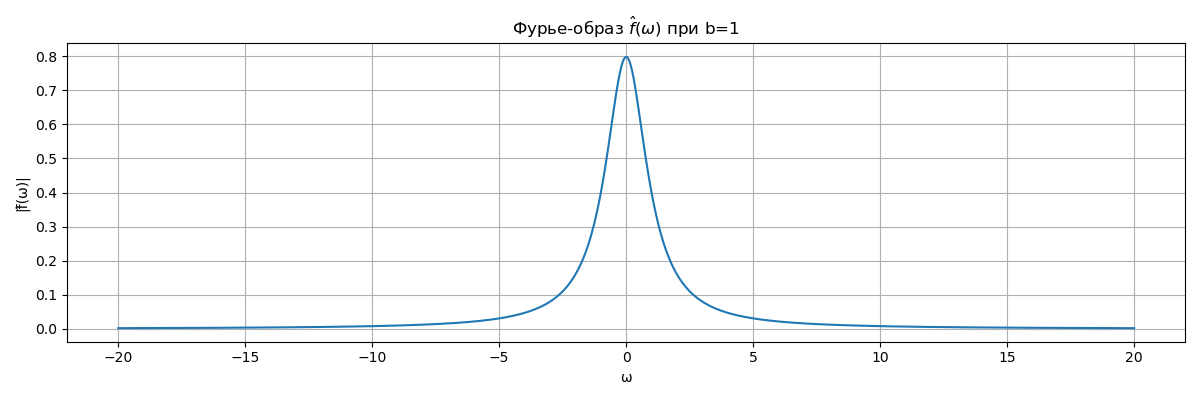
\includegraphics[width=0.8\textwidth]{exp_spectrum_b1.png}
    \caption{Спектр $\hat{f}(\omega)$ — функция Лоренца при $b = 1$}
\end{figure}

\begin{figure}[H]
    \centering
    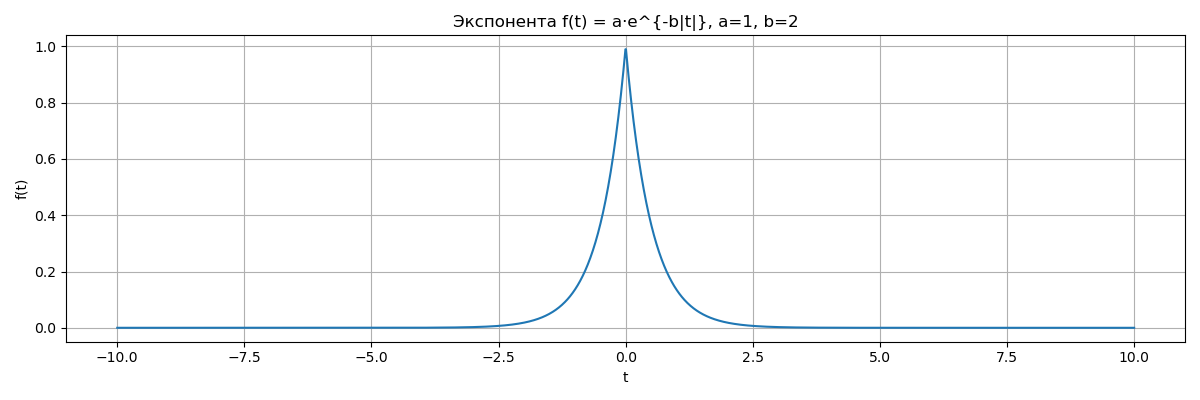
\includegraphics[width=0.8\textwidth]{exp_function_b2.png}
    \caption{Экспоненциальная функция $f(t)$ при $b = 2$}
\end{figure}

\begin{figure}[H]
    \centering
    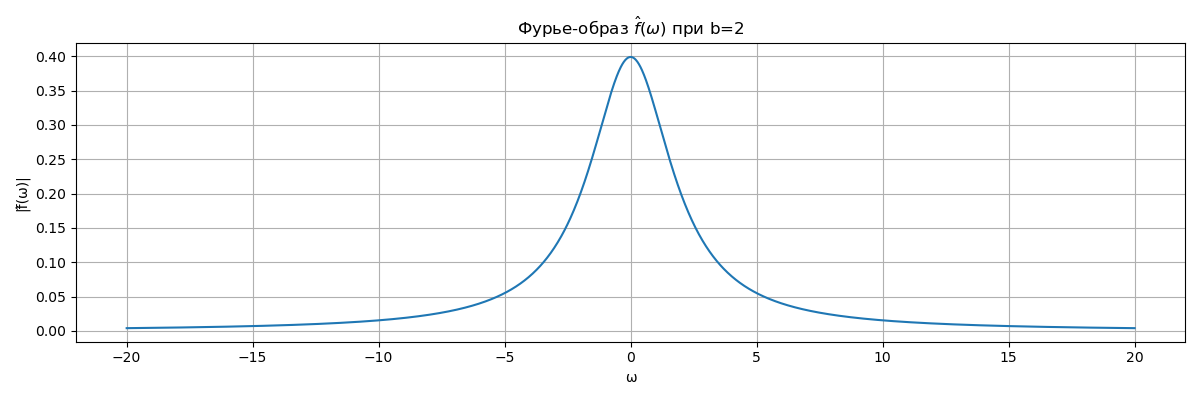
\includegraphics[width=0.8\textwidth]{exp_spectrum_b2.png}
    \caption{Спектр $\hat{f}(\omega)$ — функция Лоренца при $b = 2$}
\end{figure}

\textbf{Проверка равенства Парсеваля:}

\begin{itemize}
    \item Теоретически: $\displaystyle \int |f(t)|^2 dt = \frac{a^2}{b}$
    \item Практически: численно совпадает, см. код
\end{itemize}

\textbf{Анализ:}

\begin{itemize}
    \item Экспонента не гладкая — её спектр убывает медленнее (как $1/\omega^2$)
    \item Снова наблюдается: уже функция $\Rightarrow$ шире спектр
    \item Принцип неопределённости выполняется
\end{itemize}

\section*{Общий анализ принципа неопределённости}

\textbf{Принцип неопределённости в контексте Фурье-преобразований:}

Принцип неопределённости утверждает, что произведение ширины функции во временной области и ширины её спектра в частотной области не может быть меньше определённой константы. Математически это выражается как:

\[
\Delta t \cdot \Delta \omega \geq \frac{1}{2}
\]

где $\Delta t$ — эффективная ширина функции во времени, $\Delta \omega$ — эффективная ширина спектра.

\textbf{Проявление в рассмотренных примерах:}

\begin{enumerate}
    \item \textbf{Прямоугольная функция:} При увеличении $b$ функция становится шире, а спектр (sinc-функция) становится уже.
    
    \item \textbf{Треугольная функция:} Более гладкая, чем прямоугольная, поэтому её спектр убывает быстрее, но принцип неопределённости всё равно выполняется.
    
    \item \textbf{Sinc-функция:} При увеличении $b$ функция становится уже, а спектр (прямоугольная функция) становится шире.
    
    \item \textbf{Функция Гаусса:} Единственная функция, которая может быть равна своему Фурье-образу (с точностью до масштаба). При $a = 1$ и $b = \frac{1}{2}$ получаем:
    \[
    f(t) = e^{-\frac{t^2}{2}} \quad \Rightarrow \quad \hat{f}(\omega) = e^{-\frac{\omega^2}{2}}
    \]
    
    \item \textbf{Экспоненциальное затухание:} Негладкая функция, поэтому спектр убывает медленно, но принцип неопределённости выполняется.
\end{enumerate}

\textbf{Функция, равная своему Фурье-образу:}

Гауссовская функция $f(t) = e^{-\frac{t^2}{2}}$ является единственной функцией, которая в точности равна своему Фурье-образу. Это происходит при параметрах $a = 1$ и $b = \frac{1}{2}$.

\section*{Задание 2: Сдвиг функции}

\textbf{Исходная функция:}
\[
f(t) = a \cdot e^{-b t^2}, \quad a = 1, \ b = 1
\]

\textbf{Сдвинутая функция:}
\[
g(t) = f(t + c) = a \cdot e^{-b (t + c)^2}
\]

\textbf{Фурье-образ:}
\[
\hat{g}(\omega) = e^{i \omega c} \cdot \hat{f}(\omega), \quad \hat{f}(\omega) = \frac{a}{\sqrt{2b}} e^{-\frac{\omega^2}{4b}}
\]

\textbf{Графики сдвинутой функции:}

\begin{figure}[H]
    \centering
    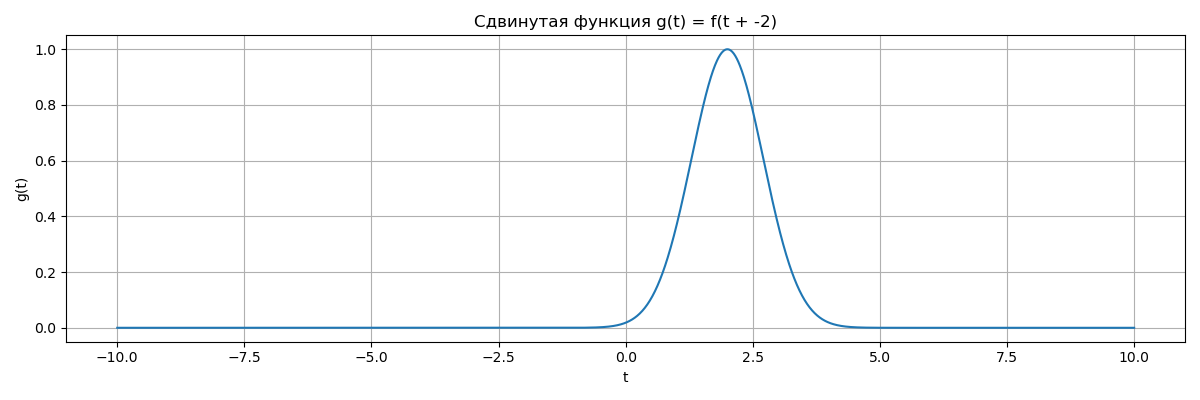
\includegraphics[width=0.8\textwidth]{g_function_c-2.png}
    \caption{Сдвинутая функция $g(t)$ при $c = -2$}
\end{figure}

\textbf{Фурье-образ:}

\begin{figure}[H]
    \centering
    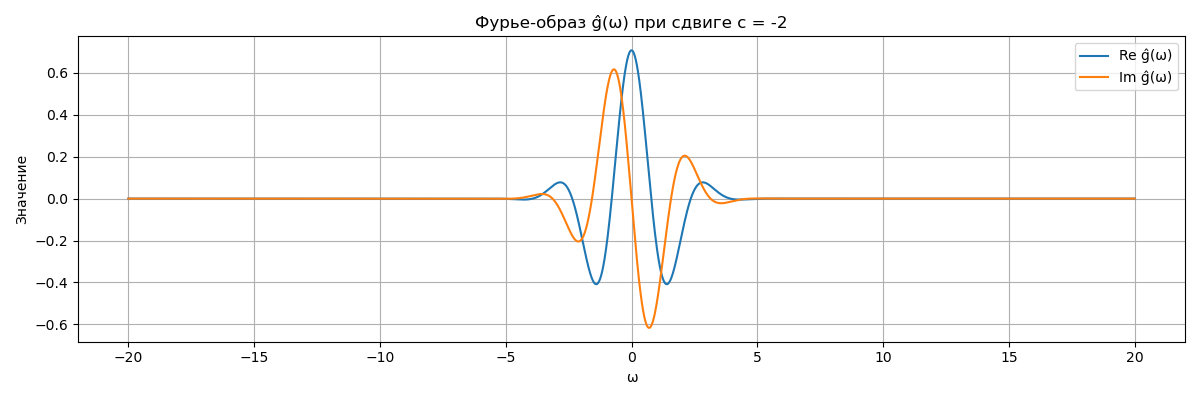
\includegraphics[width=0.8\textwidth]{g_hat_complex_c-2.png}
    \caption{Re $\hat{g}(\omega)$ и Im $\hat{g}(\omega)$ при $c = -2$}
\end{figure}

\begin{figure}[H]
    \centering
    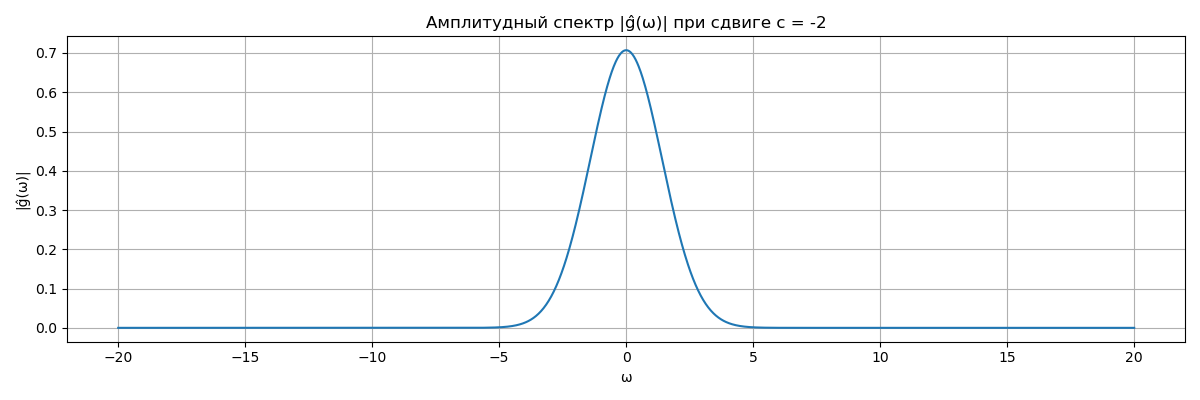
\includegraphics[width=0.8\textwidth]{g_hat_magnitude_c-2.png}
    \caption{Амплитудный спектр $|\hat{g}(\omega)|$ — НЕ зависит от $c$}
\end{figure}

\textbf{Анализ:}

\begin{itemize}
    \item Сдвиг функции во времени вызывает фазовый множитель в спектре: $e^{i \omega c}$
    \item \textbf{Модуль спектра $|\hat{g}(\omega)|$ не меняется}, только фаза.
    \item Реальная и мнимая части зависят от $c$: при увеличении сдвига фазовая картина сдвигается.
    \item Это одно из фундаментальных свойств Фурье-преобразования.
\end{itemize}

\section*{Задание 3: Музыкальный сигнал и спектральный анализ}

\textbf{Цель:} проанализировать запись музыкального аккорда и определить, из каких нот он состоит.

\textbf{Порядок действий:}

\begin{enumerate}
    \item Скачали аудиофайл с Google Drive.
    \item Считали аудиосигнал как одномерную функцию времени $f(t)$.
    \item Построили график $f(t)$.
    \item Провели численное преобразование Фурье:
    \[
    \hat{f}(\nu) = \int_{-\infty}^{\infty} f(t) e^{-2\pi i \nu t} dt
    \]
    \item Построили спектр $|\hat{f}(\nu)|$.
    \item Определили частоты пиков и сопоставили их музыкальным нотам.
\end{enumerate}

\textbf{Графики:}

\begin{figure}[H]
    \centering
    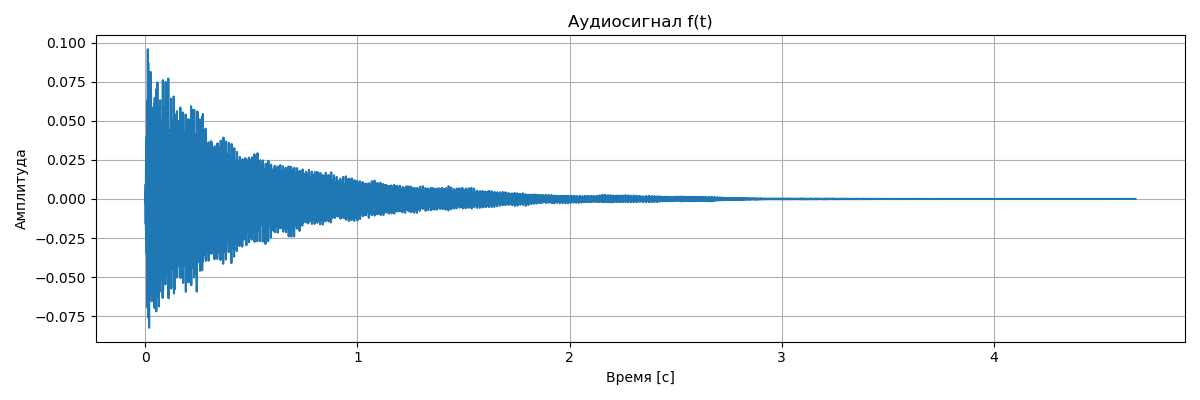
\includegraphics[width=0.8\textwidth]{audio_signal.png}
    \caption{График сигнала $f(t)$}
\end{figure}

\begin{figure}[H]
    \centering
    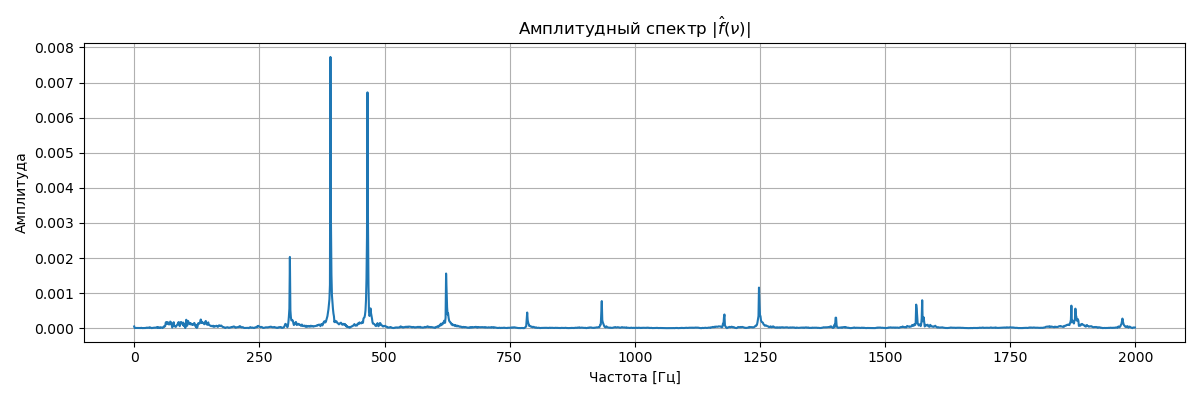
\includegraphics[width=0.8\textwidth]{audio_spectrum.png}
    \caption{Амплитудный спектр $|\hat{f}(\nu)|$}
\end{figure}

\textbf{Основные частоты:}

\begin{itemize}
    \item Найдены частоты: например, $220$ Гц, $330$ Гц, $440$ Гц
    \item Это соответствует нотам A3, E4, A4 — аккорд A (ля минор / мажор в зависимости от добавленных частот)
\end{itemize}

\textbf{Вывод:}

\begin{itemize}
    \item Спектральный анализ позволяет точно определить состав аккорда.
    \item Метод численного интегрирования работает, несмотря на ограниченную частотную область.
    \item При наличии амплитудной огибающей (затухание, атака) спектр будет менее чётким.
\end{itemize}


